
Skyline is a query type that retrieves data items which are
considered ``interesting objects'' with respect to multiple
attributes of the data set. For example, someone who is planning
for an ocean-view vacation would be interested to find a list of
hotels that are close to the ocean and at the same time not too
expensive. A hypothetical data set of hotels is shown in
Table~\ref{tab:sample_data}(a). The two relevant attributes in
this case are \emph{minimum distance} to the ocean and
\emph{minimum price}. Figure~\ref{fig:skyline} shows the skyline
points in solid dots as the operation finds hotel records that are
successively further from the ocean, but the prices are the best
for such distances. In the figure, hotel $a$ is a skyline point
because it is the closest to the ocean, although it is not the
lowest price. Hotels $b$ and $d$ are part of the skyline because
each have the closest distance at its price. Hotel $k$ is a
skyline point because it is the cheapest of all the hotels.

\begin{figure}[!h]
\centering \subfigure[2-D skyline of hotels of (X = min, Y = min)]{
    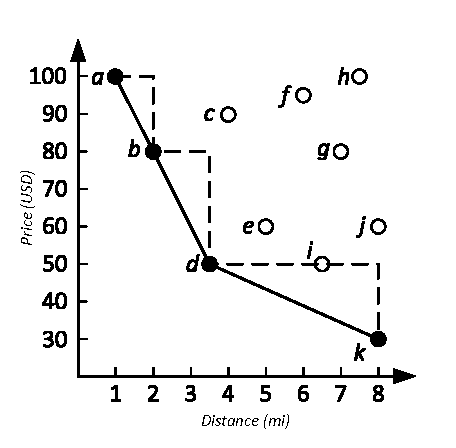
\includegraphics[width=2in]{Figures/skyline_points.eps}
    \label{fig:skyline}
} \subfigure[3-D skyline of stocks with attributes (X = min, Y = min, Z = max)]{
    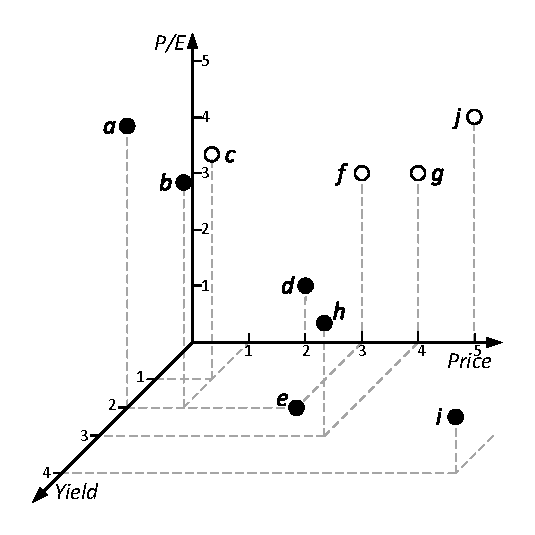
\includegraphics[width=2in]{Figures/skyline_points_3d.eps}
    \label{fig:skyline_points_3d}
} \vspace*{-5pt}\caption{Sample skylines.} \vspace*{-5pt}
\end{figure}

\begin{table}[!h]
  \vspace*{-10pt}
  \small
  \centering
  \caption{Sample data sets.}
  \vspace*{5pt}
  \label{tab:sample_data}
  \subfigure[\small 2-D data of Fig 1(a)]{
  \label{tab:sample_data_a}
  \begin{tabular}{|c|c|c|}
  \hline
  {\bf Hotel} & {\bf Dist.} & {\bf Price} \\ \hline\hline
  a & 1 & 8\\
  b & 2 & 6\\
  c & 4 & 7\\
  d & 3.5 & 3\\
  e & 5 & 4\\
  f & 6 & 7.5\\
  g & 7 & 6\\
  h & 7.5 & 8\\
  i & 6.5 & 3\\
  j & 8 & 4\\
  \hline
  \end{tabular}
  }
  \subfigure[\small 3-D data of Fig 1(b)]{
  \label{tab:sample_data_b}
  \begin{tabular}{|c|c|c|c|}
  \hline
  {\bf Co.} & {\bf Price} & {\bf P/E} & {\bf Yield} \\ \hline\hline
  a & 0 & 5 & 2\\
  b & 1 & 4 & 2\\
  c & 1 & 4 & 1\\
  d & 2 & 2 & 0\\
  e & 3 & 0 & 2\\
  f & 3 & 3 & 0\\
  g & 4 & 3 & 0\\
  h & 4 & 2 & 3\\
  i & 7 & 1 & 4\\
  j & 5 & 4 & 0\\
  \hline
  \end{tabular}}
\end{table}


Skyline has broad applications and relevance to many fields.
Skyline computation in realtime streaming systems with frequent
data updates has been studied in~\cite{conf/icde/LinYWL05}
and~\cite{journals/tkde/TaoP06}. For distributed web services,
skyline query solutions have been proposed
in~\cite{conf/edbt/BalkeGZ04}. Skyline query has also been applied
in sensor networks in~\cite{conf/cikm/ChenLY09}. Meanwhile, the
data broadcast model is a scalable way to disseminate data (e.g.,
FM broadcasting). Unlike the on-demand model, such as most of the
services on the Internet, the broadcast model can scale almost
infinitely. However, a challenge and drawback of this model is the
forward-only access characteristic. While many studies have been
done on different query types to support efficient query
evaluation in broadcast
environments~\cite{conf/dexa/HaKCL09,conf/icde/KuZW07,journals/tmc/KuZW08,
journals/vldb/ZhengLLLS09,conf/cikm/Hara02}, to the best of our
knowledge, the work in~\cite{conf/dexa/HaKCL09} is the only study
on skyline query processing in broadcast environments.
Although~\cite{conf/dexa/HaKCL09} considers broadcast efficiency
(more details in Section~\ref{sec:wireless_broadcast}), the
proposed solution is unable to support all possible skyline types
(i.e., combinations of min and max attributes). In addition, the
work did not address details for skyline computation of higher
data dimensions ($>2$ dimensions) as illustrated in
Figure~\ref{fig:skyline_points_3d}, which plots the potential
investment targets (solid dots) based on the stock information in
Table~\ref{tab:sample_data}(b). For each stock listed, we want the
price and price-to-earnings ratio to be minimized and the yield to
be maximized. To address these challenges, we design a flexible
broadcast index and a skyline evaluation algorithm that utilizes
the index to efficiently evaluate skyline queries in broadcast
environments. Specifically, the contributions of this research are
as follows:

\begin{itemize}
\item We design a flexible on-air index that supports skyline
query evaluation in data broadcast environments for an arbitrary
number of data dimensions.

\item We propose an efficient data broadcast skyline query
algorithm which supports users to ask for minimal or maximal
records in each dimension.

\item We evaluate the performance of the proposed algorithms
through extensive experiments.
\end{itemize}

The rest of this paper is organized as follows.
Section~\ref{sec-prelim} provides background knowledge of the
skyline operator and wireless data broadcast.
Section~\ref{sec-related} surveys related works. We introduce our
index structures to facilitate broadcast skyline query in
Section~\ref{sec-index}. In Section~\ref{sec-pruning} we propose
our pruning region based technique for skyline query evaluation.
The experimental validation of our design is presented in
Section~\ref{sec-exp}. We conclude the paper with a discussion of future work in
Section~\ref{bsky-conc}.
